%\chapter{3HDM}
%\label{ch:3HDM}

\newpage 

\chapter{Proper 3HDM}

%\section{Context}

% The BGL Model. Historical Contex 
% 
% The rho paramater. 
% 
% Skipping most things. 

As referenced, one of the simplest ways to expand the SM is to add elements to it's scalar sectors, on the previous example a complex scalar field originated a additional neutral scalar in harmony with a new gauge boson.
%
Now we will move on to another sort of BSM scenario, 
%
%in particular one Model called the three Higgs Doublet Model (3HDM). 
%
a three Higgs Doublet Model (3HDM). 
%
This model contains in parallel with the standard SM Higgs doublet two additional replicas of that same doublet, together these form a sort of family in the scalar sector. 
%
This addition creates a analogy to the fermion sector. This idea is far from original and was first discussed by Weinberg in, \cite{Weinberg1976}.
% 
Naturally all these Higgs doublets will take a VEV value in the same shape as the SM. 
%
The additional Higgs doublet would not alter the tree-level electroweak $\rho$ parameter as long the condition that the sum of the doublet VEVs are equal the value for the electroweak VEV in case of the SM {\color{blue} citation needed}. 
%
These conditions are a natural imposition in these models. 

The first model that attempted to perform a doublet based extension 
was the Two Higgs Doublet Model (2HDM) proposed by T.D. Lee \cite{Lee1973}.  
%
%Although a footnote in our work, we will briefly present the background of the studies surrounding the 2HDM model. 
%
His work motivated by the search for a spontaneous breaking of the CP symmetry. 
%
A great deal of interest was invested in 2HDMs, given their possible dark matter candidates large particle spectrum, including charged and additional neutral scalars.
%
However in most structures the possibility of tree-level scalar mediated FCNCs emerged. 
% 
A analysis of their origin led to disturbing conclusions, given the fermions now have their mass generated by several Yukawa matrices their simultaneous diagonalization wasn't guaranteed. 
%
These tree-level FCNCs are in direct opposition to experimental results and would need to be suppressed. 
%
Consulting the literature, as in, \cite{Branco:1999fs}, we see this forces the extra scalars to have masses above 1 TeV.  
%
%From this analysis a very disturbing conclusion is reached, from the addition of extra scalar doublets the fermions of a particular charge receive their mass from multiple Yukawa matrices and hence their diagonalization can not be ensured. The fact the Yukawa matrices can't be simultaneously diagonalized leads to FCNCs mediated by scalars. This is in direct opposition to experimental results unless heavily suppressed. Thus we can consult the literature in \cite{Branco:1999fs} and see this forces the extra scalars to have masses above 1 TeV.  
%
These heavy scalars although a possibility given current observations, are far from ideal, since there is no indication such heavy scalars exist. 
%
Several mechanisms and adjustments were made to try to deal with the tree-level FCNC problem. First, in, \cite{Ferreira_2011,Nebot_2015,ferreira2019strong}, it is proposed a framework in which we have the balancing of CP-odd and CP-even contribution to FCNCs, however, this would requires some fine-tuning, making it very unappealing. 
%
%Ideally we would like to see lighter scalars, so several mechanisms have been proposed to allow for the study of 2HDM models at lower masses while. First, balencing the CP-odd and CP-even contribution to FCNCs could allow for a lighter scalar sector, see, \cite{Ferreira_2011,Nebot_2015,ferreira2019strong}.  
% 
Another possibility is to assume alignment between different Yukawa matrices such that no FCNCs are present, see \cite{Pich_2009,Jung_2010,Jung_2011} for more information. 
%
Finally we could also use the approach presented in the BGL (Branco-Grimus-Lavoura) version of the 2HDM \cite{Branco_1996,LAVOURA1994}, here the authors impose a flavour-violating symmetry naturally keeping the FCNCs under control trough the CKM matrix. 
%
The phenomenology of the model has been studied quite thoroughly (see, for instance \cite{Botella_2014,Botella_2016}) and it remains a possible scenario for BSM physics.
%
This BGL 2HDM is very relevant for our studies in this chapter, as we'll be presenting a 3HDM model based on a similar structure. 

In this chapter we endeavoured to look into a next-to-minimal possibility for a BGL like 3HDM framework. 
%
% The new scalars in this model include 2 neutral Higgs Bosons. 
%
We used previous work to narrow down the vast parameter space of these type of models offer, see \cite{Ferreira_2018,Ivanov_2012,Ivanov_2016,Aranda_2017}.
%
Our conclusions are consistent with these studies, where it was found to have large regions of parameter space which conformed with experimental constraints in the flavour and scalar sectors.

Our 3HDM will also contain a flavour symmetry, as to attempt to constrain the flavour observables. In particular the addition of a $\mathrm{U}(1) \times \mathrm{Z}_2$ symmetry. This symmetry constrains the terms that can appear in the flavour sector of the Lagrangian resulting in very specific structures (or textures) of the Yukawa couplings.
% achieving a similar mechanism to that of the BGL 2HDM. 
%
We hoped to prove that light scalars are still within the reach of future collider experiments in our model's framework while having FCNCs concurrent with observations. {\color{blue} Improve} 
%
We also outline the possible signatures of the nonstandard scalars present in our model that could be detected in colliders. Finally expect to show the constraints imposed upon the model, both theoretical i.e. boundedness from
below, unitarity, electroweak precision bounds. And experimental i.e. LHC Higgs data and searches for heavier scalars, flavour physics data, among others. {\color{blue} Move to top}. This was also achieve trough a numerical scan in 

\section{The formulation of a BGL-like 3HDM} 

More than the naturalist argument, there are mounting reasons to explore the possibility of a multi-doublet model, in particular the 3HDM that has been having mounting success in recent studies, see \cite{Botella_2014}, although this study shows the model's parameter space is rather constraint. 
%
Consider however that in this study the leptonic sector was also extended, something that is not necessary. { \color{blue} check if citation is a 2HDM study} 

Furthermore, challenging the 2HDM BGL paradigm could also be motivated some phenomenological comparison of the 3HDM to the 2HDM model. For example, vacuum stability in the 2HDM model can only accommodate one instance of spontaneous CP or charge symmetry breaking \cite{Branco_2012,Ferreira_2004,Barroso_2007}. 
%
However in Multiple Higgs Doublets models (NHDMs), such as the 3HDM, charge breaking minima were found to be stable while at the same time coexisting with charge-preserving ones, for more information see, \cite{Barroso_2006}.   
%
Also, for the 2HDM a full list of all possible incorporations of symmetries consistent with $\mathrm{SU(2)}\times\mathrm{U(1)}$ has been achieved \cite{Ivanov_2008,Ivanov2007}, while for the 3HDM no work has thus far been compleated, see, \cite{Ivanov_2012,Ivanov_2015}. 
%
Moreover generic unitarity constraints have been found for the 2HDM \cite{Ginzburg_2005} but not for 3HDMs. As such, the possibility of
ascertaining whether the BGL structure can be extended to a full 3HDM compels us to try to find it. 

The particle content of the model is pretty similar to the SM. Having the same gauge fields and the following fermion and scalar fields,
\begin{equation}
\begin{split}
Q_{L_i} =  \begin{pmatrix}
u_{L_i}  \\
d_{L_i}
\end{pmatrix} \quad , \quad \Psi_{L_i} =  \begin{pmatrix}
\nu_{L_i}  \\
e_{L_i}
\end{pmatrix} \\  
u_{R_i} \quad , \quad d_{R_i} \quad , \quad e_{R_i} \quad i=\{1,2,3\} \\ 
\phi_k = \begin{pmatrix}
W_k^\pm + i \, W_k^\mp \\ 
\frac{1}{\sqrt{2}}\left( v_k + h_k + i Z_k \right) 
\end{pmatrix}  \quad , \quad k=\{ 1,2,3\} 
\end{split} 
\end{equation}
where $Q_{L_i}$ , $\phi_k$ , $\Psi_{L_i}$ and $u_{R_i}$, $d_{R_i}$, $e_{R_i}$ are $\mathrm{SU}(2)_L$ doublets and singlets of the i-th and k-th
generation, respectively. These fields are all naturally charged under the new $\mathrm{U(1)}\times\mathbb{Z}_2$, one can transformation these fields as, 
\begin{equation}
\label{eq:3HDM_Transformations}
	\begin{split} 
	\mathrm{U(1)} : & \\
		& Q_{L_3} \rightarrow    e^{i \alpha} Q_{L_3}  \\  
		& u_{R_3} \rightarrow    e^{2 i \alpha} u_{R_3}  \\
		& \phi_1  \rightarrow    e^{i \alpha} \phi_1  \\   
		& \Psi_{L_1} \rightarrow e^{i \alpha} \Psi_{L_1} \\
		& \phi_3 \rightarrow     e^{i \alpha} \phi_3  \\ 
	\end{split} \quad \quad \quad  
	\begin{split}
		\mathbb{Z}_2 : & \\
		 	& Q_{L_3} \rightarrow -Q_{L_3} \\
		 	& u_{R_3} \rightarrow -u_{R_3} \\ 
		 	& \phi_1  \rightarrow -\phi_1 \\ 
		 	& \Psi_{L_1} \rightarrow - \Psi_{L_1} \\ 
		 	& \phi_3 \rightarrow -\phi_3
	\end{split} 
\end{equation} 
%
This symmetry will have to be softly broken as to avoid the appearance of a massless Goldstone state. All remaining fields not shown in Eq. \ref{eq:3HDM_Transformations} remain unchanged under transformations of the $\mathrm{U(1)}\times\mathbb{Z}_2$ global symmetry. 
\subsection{Introducing a Scalar Sector}

Let us then start our proper introduction to the workings of the model by presenting the scalar sector where the new spin-0 $\mathrm{SU(2)}$ doublets, $\phi_i$, $i=\{1,2,3\}$ reside. 
\begin{comment}
The scalar doublets are made to transform under the imposed $\mathrm{U(1)}\times \mathbb{Z}_2$ symmetries as, 
%
\begin{equation}
\begin{split}
\mathrm{U(1)} & : \phi_1 \rightarrow \phi_1 e^{i \alpha} \quad ,
            \quad \phi_3 \rightarrow \phi_3 e^{i \alpha}  \\
\mathbb{Z}_2  & : \phi_1 \rightarrow -\phi_1 \ \ \quad , 
            \quad \phi_2 \rightarrow \phi_2  \quad , 
            \quad \phi_3 \rightarrow \phi_3 \quad .
\end{split}
\end{equation}
\end{comment}
Note the scalar potential to be CP-invariant, this means,
\begin{equation}
\phi_1 = \phi_1^{\**} \quad , \quad \phi_2 = \phi_2^{\**} \quad , \quad 
\phi_3 = \phi_3^{\**} 
\end{equation}
The generic scalar potential that follows all these transformations is extensively written in, 
\begin{equation}
\begin{split}
V(\phi_i) = & 
- \mu_1^2 \left( \phi^{\dagger}_1 \phi_1 \right) 
- \mu_2^2 \left( \phi^{\dagger}_2 \phi_2 \right)  
- \mu_3^2 \left( \phi^{\dagger}_3 \phi_3 \right) \\ 
& - \mu_{13}^2 \left( \phi^{\dagger}_1 \phi_3  \right) 
  - \mu_{23}^2 \left( \phi^{\dagger}_2 \phi_3  \right)  
  - \mu_{21}^2 \left( \phi^{\dagger}_2 \phi_1  \right)  \\
& + \lambda_1 \left( \phi^{\dagger}_1 \phi_1 \right) 
  + \lambda_2 \left( \phi^{\dagger}_2 \phi_2 \right)  
  + \lambda_3 \left( \phi^{\dagger}_3 \phi_3 \right) \\  
& + \lambda_4 \left( \phi^{\dagger}_1 \phi_1 \right)  \left( \phi^{\dagger}_2 \phi_2 \right) 
  + \lambda_5 \left( \phi^{\dagger}_1 \phi_1 \right)  \left( \phi^{\dagger}_3 \phi_3 \right)  
  + \lambda_6 \left( \phi^{\dagger}_2 \phi_2 \right)  \left( \phi^{\dagger}_3 \phi_3 \right)  \\ 
& + \lambda_7 \left( \phi^{\dagger}_1 \phi_2 \right)  \left( \phi^{\dagger}_1 \phi_2 \right)  
  + \lambda_8 \left( \phi^{\dagger}_1 \phi_3 \right)  \left( \phi^{\dagger}_3 \phi_1 \right)   
  + \lambda_9 \left( \phi^{\dagger}_2 \phi_3 \right)  \left( \phi^{\dagger}_3 \phi_2 \right)  \\
& + \lambda_{10} \Bigg\{ \left( \phi^{\dagger}_1 \phi_3 \right)^2 + \text{h.c.} \Bigg\}   
\end{split} 
\end{equation}
Recall that due to the CP symmetry imposed on this potential all parameters, $(\lambda_i,i=\{1,...,10\})$, here are real.
%
The parameter $\mu_{23}$ was added as to impede the formation of a massless axion. 
% 
For the scalar potential $V$ to have a stable vacuum it needs to satisfy \textit{boundness from below} conditions. 
%
As before this will ensure that there is indeed an absolute minimum of energy. 
%
To solve these one must write the derivates of the potential with respect to the fields as,
%
\begin{equation}
\label{eq:3HDM_tadpoles}
\begin{split}
\frac{\partial V}{\partial \phi_1} = & \frac{1}{2} v_1 \left( \left( 2 \lambda_{10} + \lambda_5 + \lambda_8 \right) v_3 + 2 \left( \lambda_1 v_1 + \mu_1^2 \right) + \left( \lambda_4 + \lambda_7 \right)  \right)  \\ 
\frac{\partial V}{\partial \phi_2} = & \frac{1}{2} v_2 \left( 2\left( \lambda_2 v_2^2 + \mu_2^2 \right) + \left( \lambda_4 + \lambda_7 \right) v_1^2 + \left( \lambda_9 + \lambda_6 \right)v_3^2 \right) + \mu_{23} v_3 \\
\frac{\partial V}{\partial \phi_3} = & \frac{1}{2} \left( \left( 2 \lambda_{10} + \lambda_5 + \lambda_8  \right) v_1^2  + 2 \mu_3^2 + \left( \lambda_6 + \lambda_9 \right) v_2^2 \right) v_3 + \lambda_3 v_3^3 + \mu_{23}^2 v_2 \\
\end{split} 
\end{equation}
%
By requiring that the derivatives of the potential vanish for some value of the CP-even fields $\phi_i$ , one arrives at the so-called tadpole equations of the model.
%
{\color{red} Should I explain further?} 

After the process of SBB, all Higgs doublets take a VEV shape similar to that of the SM Higgs, written as, 
%
\begin{equation}
\phi_k = 
\begin{pmatrix}
W_k^\pm + i \, W_k^\mp \\ 
\frac{1}{\sqrt{2}}\left( v_k + h_k + i Z_k \right)
\end{pmatrix}  \rightarrow \langle \phi_k \rangle = \begin{pmatrix}
0 \\ 
\frac{v_k}{\sqrt{2}}
\end{pmatrix} \quad , \quad k=\{ 1,2,3\} 
\label{shame}
\end{equation} 
Where the sum of the VEVs must satisfy, 
\begin{equation}
\label{eq:VEV_Condition}
\sum_{k=1}^3 v_k^2 = 246^2 \text{GeV}
\end{equation}
%
Given the tadpole equations from \ref{eq:3HDM_Tadpoles} we could express the quadratic terms $\mu_1$, $\mu_2$ and $\mu_3$ as follows, 
%The minimization of the potential yields three tadpole equations which means that one can express the quadratic parameters,$\mu_1$, $\mu_2$ and $\mu_3$ as follows, 
%
\begin{equation}
\label{eq:3HDM_Param_1}
\begin{split}
\mu_1^2 & = \lambda_1 v_1^2 + \frac{1}{2} \left( \lambda_4 + \lambda_7 \right) v^2_2 + \frac{1}{2} \left( \lambda_5 + \lambda_8 + 2 \lambda_{10} \right) v_2^2  \\ 
\mu_2^2 & = \lambda_2 v_2^2 + \frac{1}{2} \left( \lambda_4 + \lambda_7 \right) v_1^2 + \frac{1}{2} \left( \lambda_6 + \lambda_9 \right) v_3^2 +\frac{v_3}{v_2} \mu^2_{23}  \\
\mu_3^2 & = \lambda_3 v^2_3  + \frac{1}{2}\left( \lambda_6 + \lambda_9 \right) v^2_2 + \frac{1}{2} \left( \lambda_5 + \lambda_8 + 2 \lambda_{10} \right)v_1^2 + \frac{v_2}{v_3} \mu_{23}^2 
\end{split}  
\end{equation}
Given these Eqs. \ref{eq:3HDM_Param_1} and Eq. \ref{eq:VEV_Condition}, we can parametrize the VEVs as a function of two mixing angles $\psi_1$ and $\psi_2$, 
\begin{equation}
v_1 = v \cos(\psi_1) \cos(\psi_2) \quad , \quad v_2 = v \sin(\psi_1) \cos(\psi_2) \quad , \quad v_3 = v \sin(\psi_2)
\end{equation}
where $v=\sqrt{v_1^2 + v_2^2 + v_3^2 }$. Through this parametrization we can write the ortogonal matrix, 
\begin{equation}
\mathcal{O} = 
\begin{pmatrix}
\cos(\psi_1) \cos(\psi_2) & \cos(\psi_2) \sin(\psi_1) & \sin(\psi_2) \\ 
- \sin(\psi_1) & \cos(\psi_1) & 0 \\ 
- \cos(\psi_1) \sin(\psi_2) & \sin(\psi_1) \sin(\psi_2) & \cos(\psi_2)
\end{pmatrix}
\end{equation}
We will return to this matrix as it will be useful as we analysis the scalar, pseudoscalar and charged scalar sector. 

%$We also define the following orthogonal matrix which will simplify our analysis of the pseudoscalar and the charged scalar sectors:

\subsection{The CP-odd portion of the scalar sector}
We now turn our attention to the physical scalar spectrum of the model. 
%
This potential is explicitly CP invariant given all paramaters are real (VEVs, couplings and quadratic masses). In fact in this model we expect to find no more sources of CP-violation than in the SM. { \color{blue} ask morais if this is true } 

\subsubsection{Pseudoscalars}

The CP-odd portion of the scalar sector (related to the $z_k$ fields) contains quadratic terms after the process of SBB. These are easily extracted from the scalar potential in the form, 
%
% of quadratic terms of the $z$ fields once SBB takes place, seen as, 
\begin{equation}
V_{\text{shifted}} \supset \left( \begin{array}{ccc} z_1 & z_2 & z_3 \end{array} \right) \frac{M_P^2}{2} \left( \begin{array}{c} z_1 \\ z_2 \\ z_3 \end{array} \right)  
\end{equation}
%
where $M_P^2$ is the $3\times3$ pseudoscalar mass matrix. It can be block diagonalized as:
%
\begin{equation}
B^2_P = \mathcal{O} M_P^2 \mathcal{O}^T = \left( \begin{array}{ccc}
0 & 0 & 0 \\ 
0 & \left( B^2_P \right)_{22} &  \left( B^2_P \right)_{23} \\
0 & \left( B^2_P \right)_{32} &  \left( B^2_P \right)_{33}
\end{array} \right) 
\end{equation}
%
The line and column of zeroes in this matrix tells us that it has a zero eigenvalue which of course is the neutral Goldstone boson responsible for the Z later-on.
%
The diagonalized elements of the $B^2_P$ matrix are given by,
\begin{equation}
\begin{split}
\left( B^2_P \right)_{22} = &  \frac{ 
v_3 \left( -2 v^3_2 v_3 \lambda_10 +  v_1^2 \mu_{23}^2 \right) } 
{v_2 \left( v_1^2 + v_2^2 \right)  }  
\\
\\ 
\left( B^2_P \right)_{32} = & \left( B^2_P \right)_{23} = \frac{v_1 v \left( 2 v_2 v_3 \lambda_{10} + \mu_{23}^2 \right) }{v_2^2 + v_1^2} \\
\\
\left( B^2_P \right)_{33} = & \frac{v^2 \left( 2 v_1^2 v_3 \lambda_{10} - v_2 \mu_{23}^2 \right) }{\left( v_2^2 + v_1^2\right) v_3 }
\end{split} 
\end{equation}
From the above equations we notice that, apart from the three VEVs, only two parameters, $\lambda_10$ and $\mu_23$, enter in the pseudoscalar mass eigensystem. 
%
From here we can use the relations, 
\begin{equation}
\mathrm{Tr} ( B_P^2 ) = m_{A_1} + m_{A_2}\quad , \quad  \mathrm{Det}( B_P^2 ) =  m_{A_1}  m_{A_2}
\end{equation}
to reach the mass for the two pseudo scalars as, 

{ \color{red} ?}

\subsubsection{Charged Scalars}

Through a similar process, we can endeavour to isolate the quadratic terms relating to the charged fields as to produce a similar structure for the mass matrix of the new real charged fields, 
%
%For the case of the charged scalars, their mass generation is very similar to the generation of the pseudoscalars where a mass matrix, 
%
\begin{equation}
\label{eq:3HDM_Charged_M1}
B^2_C = \mathcal{O} M_C^2 \mathcal{O}^T = \left( \begin{array}{ccc}
0 & 0 & 0 \\ 
0 & \left( B^2_C \right)_{22} &  \left( B^2_C \right)_{23} \\
0 & \left( B^2_C \right)_{32} &  \left( B^2_C \right)_{33}
\end{array} \right) 
\end{equation}
%
Here we observe again that a line and column of zeros ensures that we have a goldstone boson leaving room for the later surge of the $W^\pm$. In the same fashion as before we define the terms of Eq.\ref{eq:3HDM_Charged_M1}, 
%
%Here we must ensure the same line and column of zeros as to assure we have a goldstone boson that will lead to the mass term of the $W$. In the same fashion as before we can find the equations for all the terms of $B^2_C$ 
%
\begin{equation}
\begin{split}
\left( B^2_C \right)_{22} & = - \frac{1}{2v_2 (v_1^2 + v_2^2 ) } \left[ v_2^5 \lambda_7 + v_2^3 \left( 2 v_1^2 \lambda_7 + v_3^2 \left( 2\lambda_{10} + \lambda_8 \right) \right)  + v_2 \left( v_1^4 \lambda_7 + v_1^2 v_3^2 \lambda_9 \right) - 2 v_1^2 v_3 \mu_{23}^2 \right]   \\ 
%
\left( B^2_C \right)_{32} & = \frac{v_1 v}{ 2 ( v_1^2 + v_2^2 ) } \left[ v_2 v_3 \left( 2\lambda_{10} + \lambda_8 - \lambda_9 \right) + 2\mu_{23}^2 \right]   \\
\left( B^2_C \right)_{33} & = \frac{v^2}{2(v_1^2 +v^2_2)v_3 }
\left[ v_1^2 v_3 \left( 2 \lambda_{10} + \lambda_8 \right) + v_2 \left( v_2 v_3 \lambda_9 - 2 \mu_{23}^2 \right) \right]   
\end{split} 
\end{equation}

{ \color{red} Power gap }

Both the equations for the diagonalized masses can be utilized to reach a parametrization of some scalar couplings,
\begin{equation}
\begin{split} 
\lambda_7 = \\
\lambda_8 = \\
\lambda_9 = 
\end{split} 
\end{equation}
Further combination with the equation for $\mu_{23}$ and $\lambda_{10}$ yields more terms of the potential expressed as a function of physical masses and respective mixing angles. 

\subsection{The CP-even portion of the scalar sector}

Following the same procedure as we did for the CP-odd portion we begin by approaching the quadratic portion of the scalar fields in the potential,
%
\begin{equation}
V \supset \left( \begin{array}{ccc} 
h_1 & h_2 & h_3 
\end{array} \right) 
\frac{M_S^2}{2} \left( \begin{array}{c}
h_1 \\ 
h_2 \\
h_3
\end{array} \right) 
\end{equation}
where $M_S^2$ is a $3\times3$ symmetric matrix. The elements of this matrix are given by,
\begin{equation}
\begin{split}
\left(M_S^2\right)_{11} & \\
\left(M_S^2\right)_{12} & \\
\left(M_S^2\right)_{13} & \\
\left(M_S^2\right)_{22} & \\
\left(M_S^2\right)_{23} & \\
\left(M_S^2\right)_{33} & 
\end{split}
\end{equation}
The physical CP scalar states that originate from this mass matrix are, $h$, $H_1$ and $H_2$, these are obtained trough a orthogonal rotation.
\begin{equation}
\left( 
\begin{array}{c}
h   \\
H_1 \\
H_2 
\end{array} 
\right) = \mathcal{O}_\alpha \left( 
\begin{array}{c}
h_1 \\
h_2 \\
h_3 
\end{array} 
\right)
\end{equation} 
Here $\mathcal{O}_\alpha$ is written as, 
\begin{equation}
\mathcal{O}_\alpha = R_1 \cdot R_2 \cdot R_3 \quad , 
\end{equation}
with, 
\begin{equation}
R_1 \quad , \quad R_2 \quad , \quad R_3 
\end{equation}
Through this $\mathcal{O}_\alpha$ we can diagonalize scalar massive eigenstates. 
\begin{equation}
\mathcal{O}_\alpha M^2_S \mathcal{O}_\alpha^T \equiv \text{diag}(m_h,m_{H_1},m_{H_2})
\end{equation}
Here we can perform another inversion, allowing us to reach a parametrization of the six remaining couplings, 
\begin{equation}
\begin{split}
\lambda_1 & \\ 
\lambda_2 & \\ 
\lambda_3 & \\ 
\lambda_4 & \\ 
\lambda_5 & \\ 
\lambda_6 & 
\end{split} 
\end{equation}

\section{Introducing the Yukawa sector}

Here in the Yukawa sector we must perform a process analogous to that carried out in the BGL like 2HDM. We must first begin by introducing the field transformations upon which the suppression of the FCNCs is derived from. This is the aforementioned $\mathcal{U(1)}\times\mathbb{Z}_2$

\begin{equation}
\begin{split}
\mathrm{U(1)} & : Q_{L_3} \rightarrow e^{i \theta} Q_{L_3} \quad , \quad p_{R_3} \rightarrow e^{2 i \theta} p_{R_3} \quad , \\ 
\mathbb{Z}_2 & : Q_{L_3} \rightarrow -Q_{L_3} \quad , \quad p_{R_3} \rightarrow - p_{R_3} \quad , \quad n_{R_3} \rightarrow - n_{R_3}
\end{split}
\end{equation}
with $\theta \neq n \pi$, with $n$ an arbitrary integer. All other fields, i.e. remaining quark fields, remain invariant under this symmetry. As in the SM left handed quarks, $Q_{L_a}=\left( p_{L_a} , n_{L_a} \right)^T$ (this denotes the left-handed quarks of the a-th generation, the up and down portion.)
%
The quark Yukawa Lagrangian for a 3HDM will take the general form, 
\begin{equation}
\mathcal{L}_Y = - \sum_{k=1}^3 \left[ \overline{Q}_{L_a} \left( \Gamma_k \right)_{ab} \sigma_k n_{R_b} + \overline{Q}_{L_a} \left( \Gamma_k \right)_{ab} \tilde{\phi}_k p_{R_b} + h.c.  \right] 
\end{equation}   
where in, $\Gamma_k$ and $\Delta_k$ stand for the Yukawa matrices for the up and down quark sectors respectively. Given the symmetry $\mathrm{U}(1)\times\mathbb{Z}_2$ this forces a very specific shape to the Yukawa matrices. We'll call these textures,
\begin{equation}
\begin{split}
\Gamma_1 & = \begin{pmatrix}
0 & 0 & 0\\
0 & 0 & 0\\
\times & \times & 0
\end{pmatrix}
\quad , \quad 
\Delta_1 = \begin{pmatrix}
0 & 0 & 0\\
0 & 0 & 0\\
0 & 0 & 0
\end{pmatrix} \quad , \\
& \\
\Gamma_2 & = \begin{pmatrix}
\times & \times & 0\\
\times & \times & 0\\
0 & 0 & 0
\end{pmatrix}
\quad , \quad 
\Delta_2 = \begin{pmatrix}
\times & \times & 0\\
\times & \times & 0\\
0 & 0 & 0
\end{pmatrix} \quad , \\ 
& \\ 
\Gamma_3 & = \begin{pmatrix}
0 & 0 & 0\\
0 & 0 & 0\\
0 & 0 & \times
\end{pmatrix}
\quad , \quad 
\Delta_3 = \begin{pmatrix}
0 & 0 & 0\\
0 & 0 & 0\\
0 & 0 & \times
\end{pmatrix} \quad . 
\end{split} 
\end{equation}
Therefore, the quark mass matrices that emerge from these Yukawa matrices have the following structure, 
\begin{equation}
M_p = \quad , \quad M_n
\end{equation}
We then rotate from the p and n fields to the physical quark states u and d via rotation matrices $V_L$ , $V_R$ , $U_L$ and $U_R$. We obtain the diagonal matrices trough this rotation just like we saw in the SM section. Trusting that we return the CKM matrix given by $V_{CKM}=V_L^\dagger U_L$.  

\section{FCNCs in the 3HDM}

Let us now analyse carefully the Yukawa couplings between the neutral scalar
eigenstates and the physical quarks, with particular attention to any FCNC couplings which may arise.

For a first approximation to the FCNC couplings, let us define the following intermediate basis for the CP-even scalars


\section{Numerical Results}

\subsection{Scalar Sector}

\subsection{Flavour}

\subsection{Fine Tuning}


\chapter{3HDM}

\section{ The $\rho$ parameter }

{ \color{green} Explain the $\rho$ paramater. meantion it increases with heavy masses, say there is the decoupling theorm. Show that more higgs doublets are supressed  } 

The rho paramater is a fraction defined by the ratio of gauge boson mass times the weinberg angle, 
\begin{equation}
\rho = \frac{M_W^2}{M^2_Z \cos(\theta_W)}
\end{equation}
\section{Pre-3HDM}
For the standard Model, at tree-level we expect this $\rho$ paramater to be exactly 1. This is exactly reproduced by experiments but provides a strong indicator for a Higgs doublet structure. 

The deviations from one stem from radiative corrections. These are very sensitive to heavy particles. 



Typical BSM scenarios that aim to fix one or more such shortcomings of the SM often end up extending the scalar
sector of the SM. In these extensions, the 125 GeV scalar observed at the LHC is not the only scalar in the spectrum but the first one in a series of others to follow.

This is an intriguing possibility which motivates us
for a closer inspection of the properties of the observed scalar and inspires us to carry on our efforts to look for
new resonances at the collider experiments.

This is often done by adding to the SM simple replicas of the SM doublet, without altering the EW VEV. The first, and unsurprisingly simplest, of these kinds of models was presented in 1973 in \cite{lee1973theory}, as a means to obtain a spontaneous breaking of the CP symmetry, and boast a rich phenomenology. Along with richer phenomenology the existence of a charged Higgs Boson allows for other phenomena to occur. {\color{red} Explain} 

\section{BGL? Should I meantion it}

The BGL model was a version of one of these 2HDM models where the scalar interactions with fermions explicitly violate flavour families. This akin to what the W boson does on the SM. This is usually avoided trough the creation of a additional $\mathrm{Z}_2$  or a $\mathrm{U}_1$ symmetry [
% S. L. Glashow and S. Weinberg, Natural Conservation Laws for Neutral Currents, Phys. Rev. D15 (1977) 1958.
% E. A. Paschos, Diagonal Neutral Currents, Phys. Rev. D15 (1977) 1966.
% R. D. Peccei and H. R. Quinn, CP Conservation in the Presence of Instantons, Phys. Rev. Lett. 38 (1977) 1440–1443
]. This forces each fermion of the same charge to couple to a single doublet, thereby preventing FCNC.

We already discussed some of the reasons why these symmetries are imposed. These tree-level mediated FCNCs would make significant contributions to the flavour sector observables, such as meson masses or the flavour decays and ratios. This would destroy the agreement with experimental observations. 

Unless the masses of the new scalars are all of order TeV, or the FCNC Yukawas couplings are fine-tuned to be very small. 

These models are meantioned here for the simple fact they propose the reason why the flavour observables are suppresed is through a aditional impossed symmetry. Thus providing a natural explination to why NP contributions to the flavour observables are to be in agreement with the SM. 

\subsection{Lagrangian Yukawa}

If we observe the quark section of the 2HDM model. We have 
%
\begin{equation}
\mathcal{L}_Y \supset \sum
\end{equation}
%
where $Q^a_L = \left( p^a_L n^a_L \right)^T$ and $\phi_i$ are the $\mathrm{SU(2)}$ weak isospin quark and Higgs doublets respectively. Here we also introduce the fields $n$ and $p$ these are the positive and negatively charged  under the $\mathcal{Z}_2$ symmetry quark fields. With $a,b$ being the family indexes for the fermion families. We have two yukawa matrices here, the coupling to the up and down sector respectively. 

Upon SSB the vaccum value of each doublet will take the shape of $\frac{v_1}{\sqrt{2}}$ and $\frac{v_2}{\sqrt{2}}$ with their sum being $246 GeV$. We define $\tan(\beta)=\frac{v_1}{v_2}$.

For a CP-conserving model we must introduce a charged scalar $H^+~$, a pseudoscalar $A$ and two CP-even scalars $h$ and $H$.  

Upon rotation to the mass basis we get the mass matrices for quarks to be, 
\begin{equation}
M_p \frac{1}{\sqrt{2}} \left( D_1 v1 + D_2 v_2 \right) \quad \frac{1}{\sqrt{2}}\left( \Gamma_1 v_1 + \Gamma_2 v_2 \right)   
\end{equation}

The eigenvalues of which will have to be the physical quakr masses. Through the same bi-unitary procedure we used earlier we can write, 
\begin{equation}
\begin{split}
D_u & = V_L^\dagger M_p V_R = diag\{ m_u , m_c ,  m_t \} \\
D_d & = U_L^\dagger M_n U_R = diag\{ m_d , m_s , m_b \}  
\end{split} 
\end{equation}
where m_x are the phsycial quark masses. These matrices like before will relate the quark states to their original fields as, 
\begin{equation}
\begin{split}
p_L & = V_l u_L \quad p_R \\
n_L & = \quad n_R 
\end{split} 
\end{equation}
The CKM matrix is then obtained as 
\begin{equation}
V= V_L U_L^\dagger
\end{equation}
We also define the following matrices, 
\begin{equation}
\begin{split}
N_u & = \frac{1}{\sqrt{2}} \\ 
N_d & = \frac{1}{\sqrt{2}}
\end{split} 
\end{equation}

which end up related to the Yukawa couplings between the physical scalars and quarks. Through these we can write the lagrangian portion of the BGL lagrangian as 
\begin{equation}
\mathcal{L}_Y = \frac{i A}{v} + \frac{h}{v} \overline{u}
\end{equation}

You can see how the lagraiang above the aligment limit is when the lightr higgs Yukawa interactions are exactly those of the SM particles. In fact if one imposses $\sin(\beta -\alpha) = 1$ this forces the vertices between h and the electroweak gauge bososns to be exactly those of the SM Higgs particle. 

In models with flavour conservation, each family  of fermions of the same electrical charge couple to a single Higgs Doublet via the impossition of the Z2 or U1 symmetry. So the diagonalization of mass matrices seen is the same as the diagonalization of the $N_u$ and $N_d$ matrices. This means that there will be no flavour violating yukawa interaction mediated by the neutral scalalars. In general it is thought that will not be case and that some FCNCs occour at the tree level. 

The BGL model is based on a symmetry impossed on the whole lagrangian that will in a sense affect only the quark and scalar fields. 
\begin{equation}
\label{EQ:transform}
Transforms of fields here. 
\end{equation}
in fact there are 6 possible choices here, depending on which family we take to be the one that transforms under these rotations.  The choise we'll examine is the one where as you can see by the \ref{EQ:transform}, is the one were the first generation of quarks is affected and this yields a peccei-Quinn scalar potential which must be complemented with a soft breaking parameter to yield a massive pseudocalar particle. 

The fermion sector sees the impact of this transformation by a set of several! entries in the Yukawa matrices that have to be set to zero. 

\begin{equation}
Showing the yukawa matrices.
\end{equation} 
Here x marks a generic non-zero entry. The form of these matricies imply a shape for the Matrix Mp that is block diagonal as,
\begin{equation}
Showing the mass matrix. 
\end{equation}
Also shaping the bi-diagonalized matrices $V_L$ and $V_R$ to be,
\begin{equation}
V_L = \quad V_R = 
\end{equation}
with some phase $\theta_r$. The shapes seen here are crucial for FCNC supression. I didn't understand but our choice leads to no FCNCs in the up sector.  


By showing a load of stuff we can see that in this case! Thus we see that the off-diagonal Yukawa couplings between scalars and down-type quarks which are indeed the strength of the FCNC interactions are CKM-suppressed. 

There is a freedom to choose the “1” family as
any one of the physical quark generations, and therefore one has three BGL models with FCNC in the down
sector and without it in the up sector. An analogous symmetry to that of eq. (8) yields another three models,
where FCNC now occurs associated with a given family of up-type quarks but where no FCNC occurs for
down-type quarks.

This then is how the hallmark of the BGL models is achieved: a flavour-breaking symmetry, which yields off-
diagonal FCNC couplings naturally suppressed by the entries of the CKM matrix elements. We will now build
a similar model, but with three Higgs doublets


\section{General Notes}

\subsection{Basic}

Here we discuss the construction a three Higgs doublet model with a flavour non-universal $\mathrm{U(1)}\times\mathrm{Z_2}$. This symmetry will suppress the flavour changing interactions mediated by neutral scalars. 

such a model can thus encourage direct searches for extra Higgs bosons in the future collider experiments, and includes a
non-trivial flavour structure.

Beyond the simply aesthetic considerations of having 3 Higgs doublets as we have 3 generations of fermions there is a large range of reasons why the attempt of a 3HDM with similar suppression of FCNCs as in the BGL models. (which?) 

The BGL model was quite unique and successful but recent studies have shown that it's parameter space is quite limited. Although these studies did not consider the leptonic sector and how these sectors interact with the extended scalar family [
%[arXiv:1401.6147]
]

BGL models have enough freedom to have a flavour-preserving leptonic sector in what concerns the scalars, which is what we will consider here. Nonetheless, this shows that even with natural FCNC coupling suppression via off-diagonal CKM matrix elements. 

\section{Formulation of the 3HDM-BGL like model}

\subsection{The scalar potential}

The scalar doublets are made to transform under the $U(1) \times Z_2$ symmetry as follows: 
\begin{equation}
Transformations 
\end{equation}
We must require the scalar potential to be CP-invraiant, this means to be invariant under CP transformations. 
\begin{equation}
more transformations
\end{equation}
Then given this the scalar potential takes shape,
\begin{equation}
V(\phi)
\end{equation}
Where due to the CP symmetry all parameters are real. We have introduced a real soft breaking term with the parameter $\mu$ to avoid the appearance of a massless axion. The same process as in the 2HDM BGL due to the similar breaking of the $U(1)$ symmetry. 

All doublets acquire the same shape after their  VEV aquisition, 
\begin{equation}
VEV Shape 
\end{equation}
where vk represnets the VEV of each doublet, these must satisfy the condition $\sum = (246 GeV)^2$ The minimization of the potential yields three equations which means that one can express the quadratic parameters  $\mu_i$ in favour of these VEV and couplings as, 
%
\begin{equation}
\mu_s eqs 
\end{equation}
%
We also parameterize the VEVs as
%
\begin{equation}
vs = 
\end{equation}
%
where v is just the value of the electroweak vev. The orthogonal matrix, 
%
\begin{equation}
\mathcal{O}
\end{equation}
%
Will simplify our analysis of the charged and pseudoscalar sectors. We turn our attention to the physical scalar spectrum of the model. Since we are considering a potential with explicit CP ocnservation and a vacum who does not break CP. the neutral scalars have definite CP quantum numbers and the scalar spectrum of the model is composed of a trio of cP even scalars and a pair of charged scalars. 

\subsubsection{The CP-odd scalar sector}

\subsubsection{The CP-even or charged scalar sector}

\subsection{The Yukawa sector}

\subsection{The inverse procedure and the Quark masses}

\section{Constraints on the Model}

\section{Numerical Results}

\subsubsection{Higgs Plots}


%%%%%%%%%%%%%%%%%%%%%%%%%

\begin{figure}[H]
	\centering
	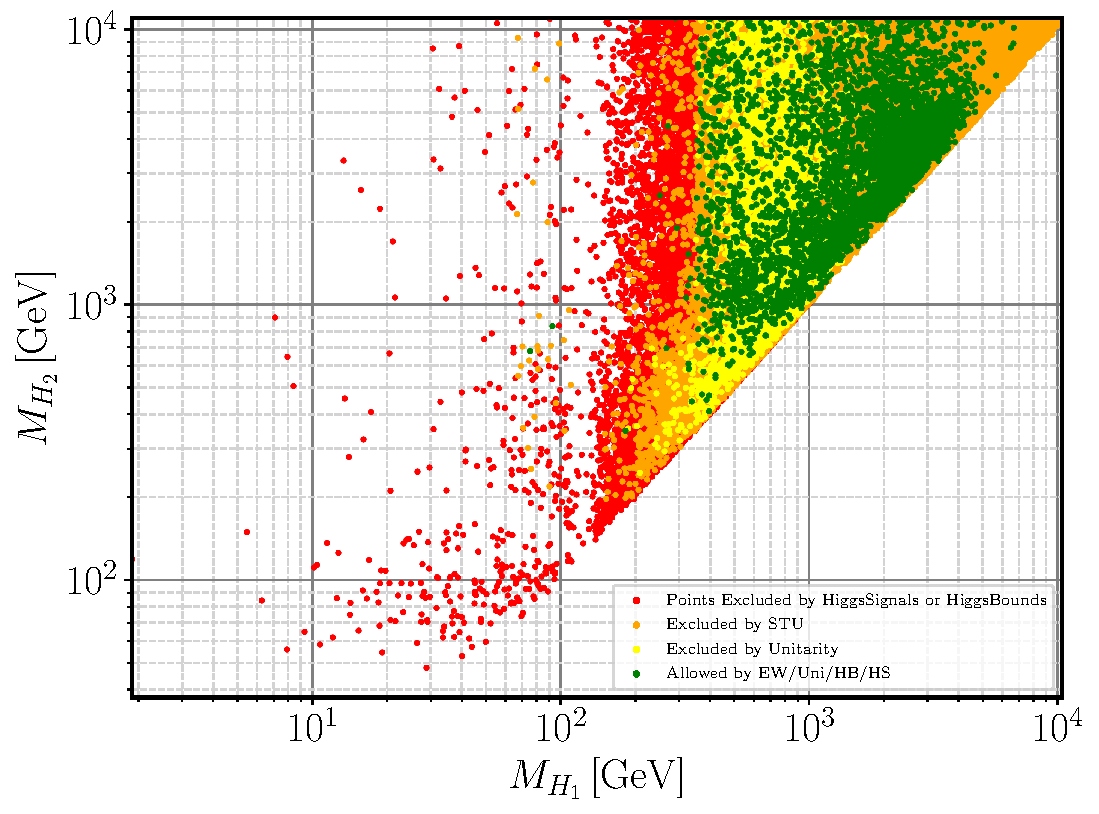
\includegraphics[width=.49\textwidth]{/3HDM/H1_H2.pdf}
	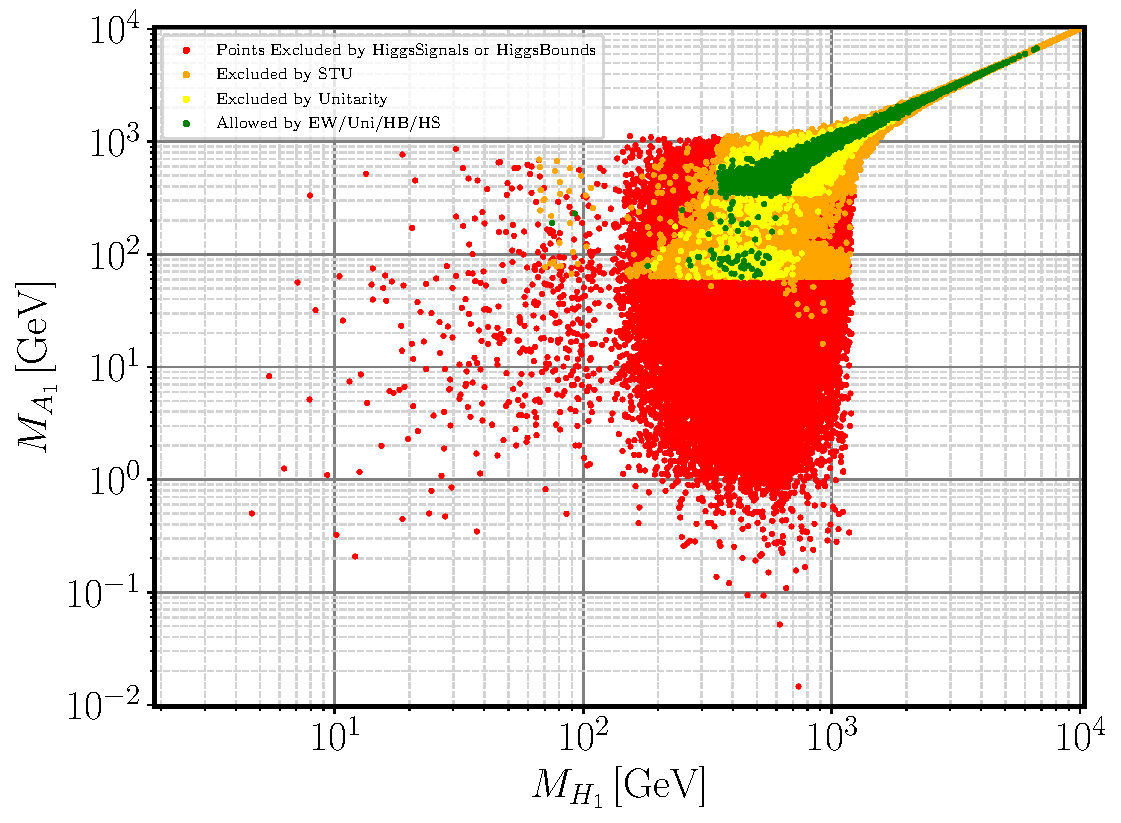
\includegraphics[width=.49\textwidth]{/3HDM/H1_A1.pdf}
	\caption{Scatter plots of parameter space allowed under  several cuts imposed on the BGL-like 3HDM. Right we have the plot showing the masses of the two heavier CP-even scalars $H_2$ and $H_1$ while in the right we show the relation between the lightest
(non-h) of the CP-even and pseudoscalar particles. Red points failed HS and HB tests; yellow points violate unitarity constraints; orange points only fail electroweak precision constraints, and green ones satisfy all restrictions.}
	\label{fig:H1_A1_Plots}
\end{figure}	

\begin{figure}[H]
	\centering
	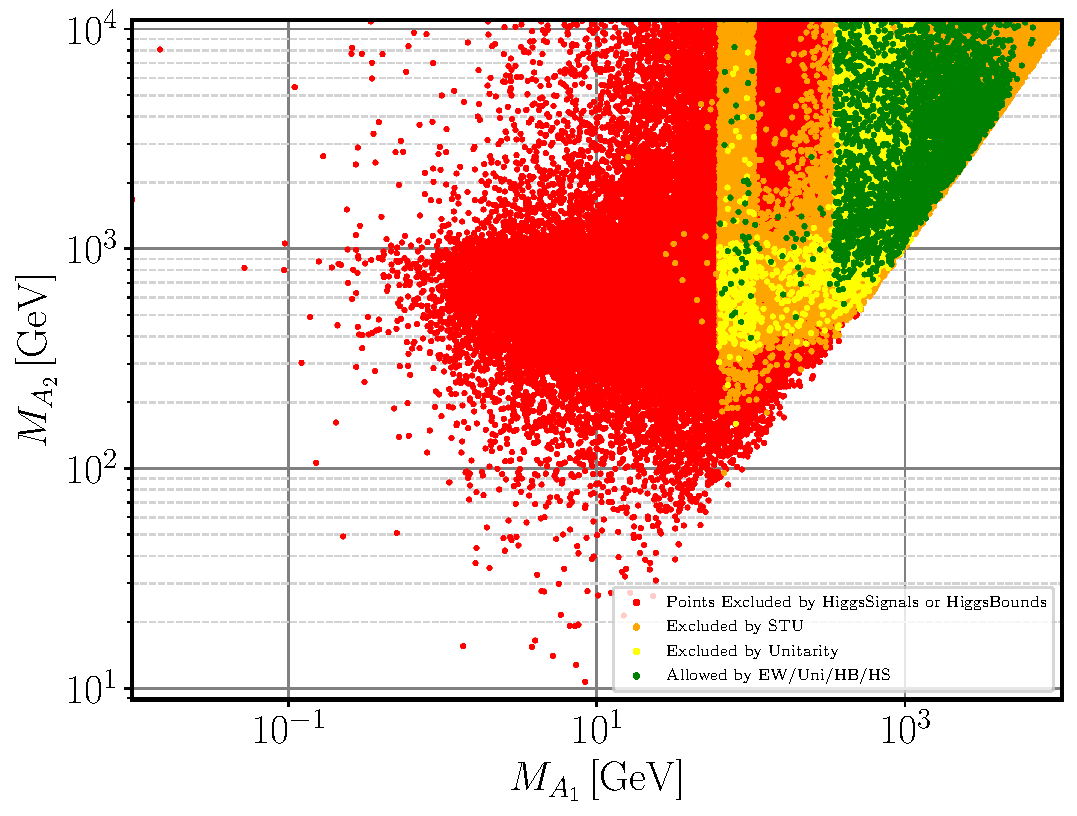
\includegraphics[width=.49\textwidth]{/3HDM/A1_A2.pdf}
	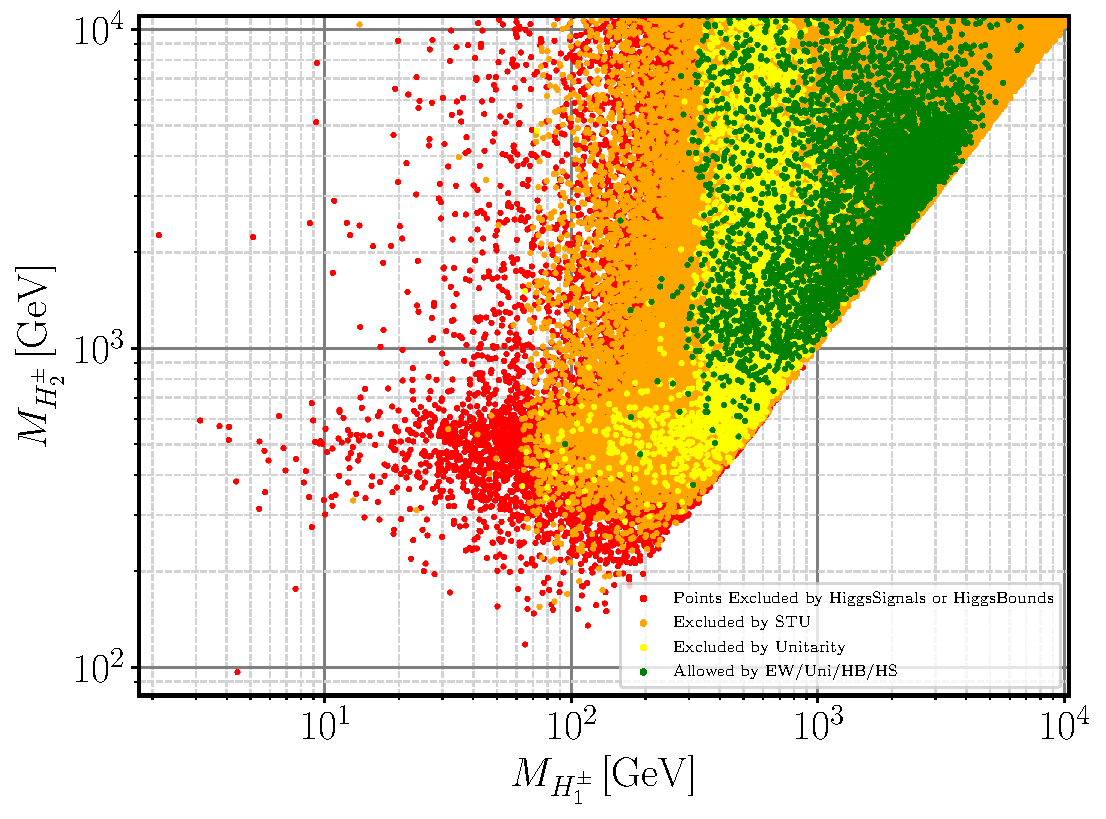
\includegraphics[width=.49\textwidth]{/3HDM/Hc1_Hc2.pdf}
	\caption{}
	\label{fig:Other_H_plots}
\end{figure}	
%
O
%
\subsection{Flavour results}

\begin{figure}[H]
	\centering
	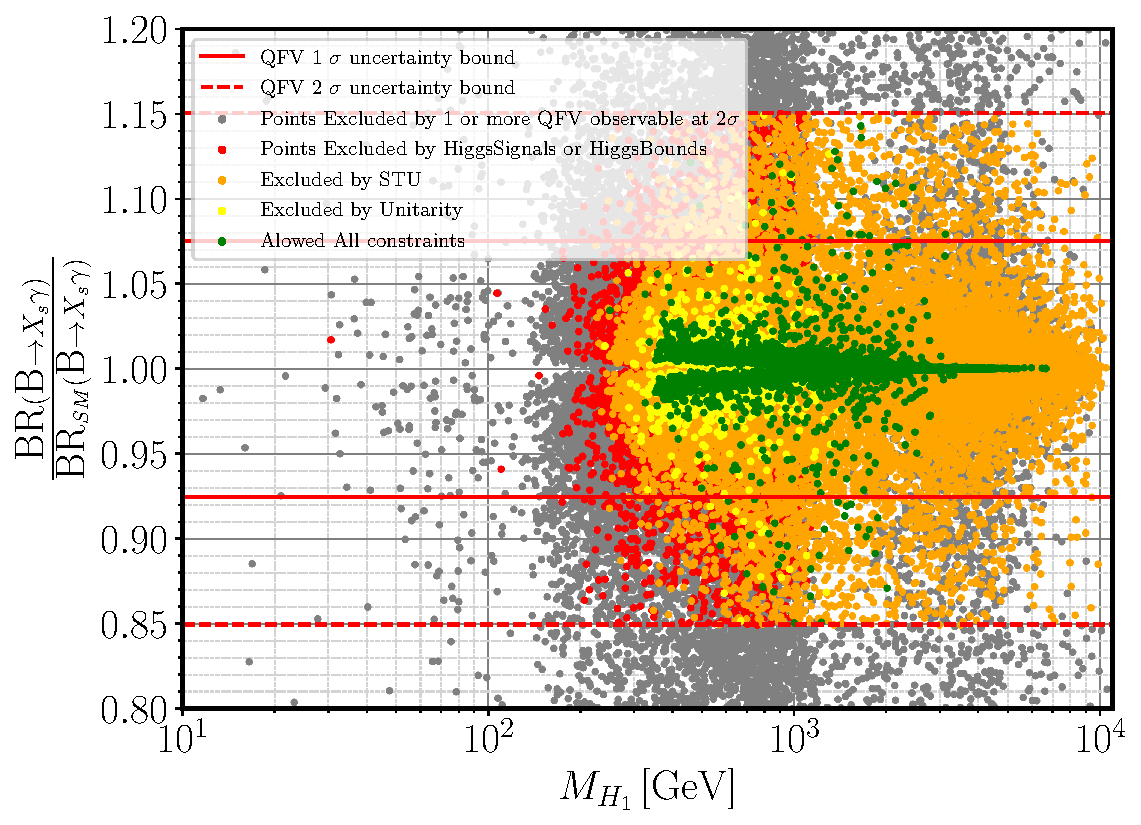
\includegraphics[width=.49\textwidth]{/3HDM/XsGamma_H1.pdf}
	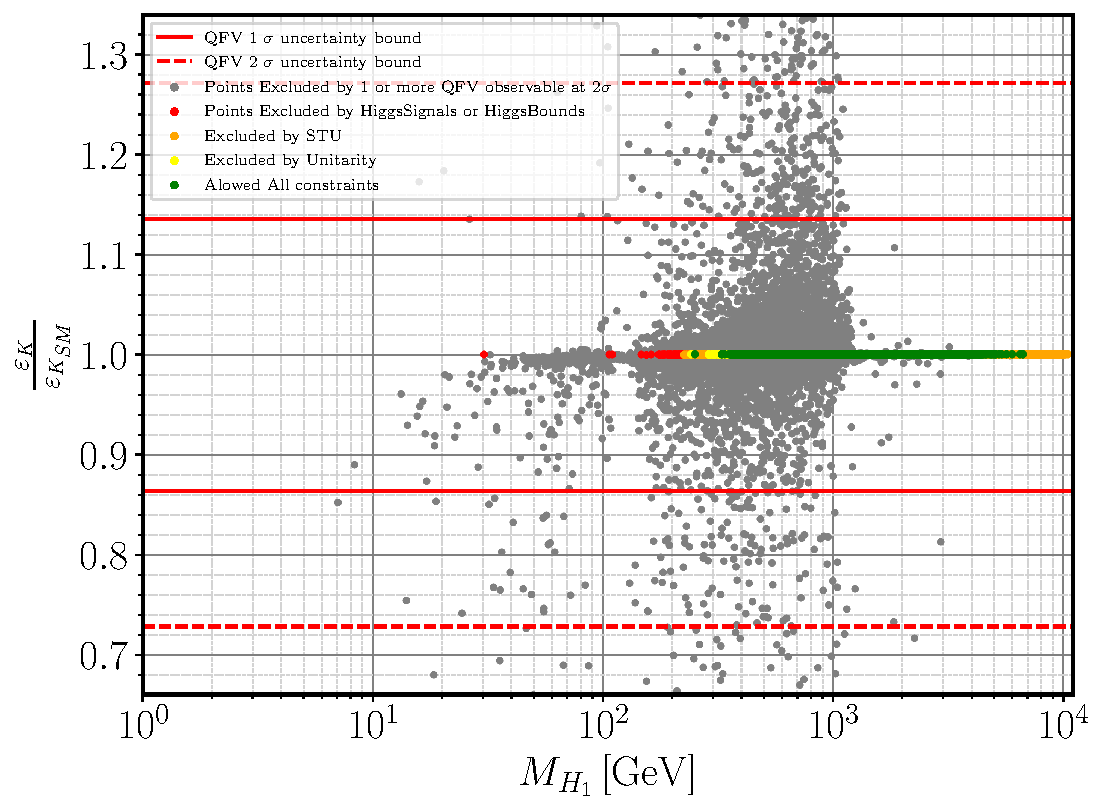
\includegraphics[width=.49\textwidth]{/3HDM/Eps_K_H1.pdf}
	\caption{Scatter plots of parameter space allowed under  several cuts imposed on the BGL-like 3HDM. Right we have the plot showing the masses of the two heavier CP-even scalars $H_2$ and $H_1$ while in the right we show the relation between the lightest
(non-h) of the CP-even and pseudoscalar particles. Red points failed HS and HB tests; yellow points violate unitarity constraints; orange points only fail electroweak precision constraints, and green ones satisfy all restrictions.}
	\label{fig:PT_plots_H1}
\end{figure}	


\begin{figure}[H]
	\centering
	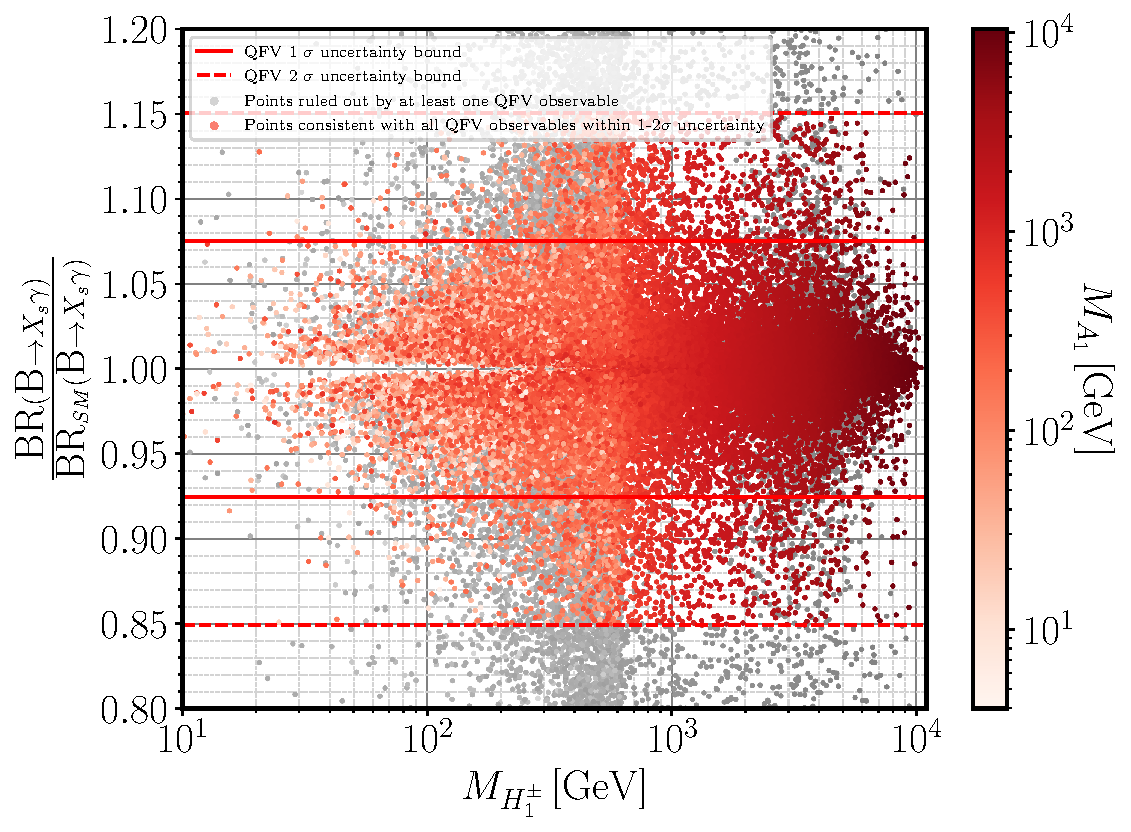
\includegraphics[width=.75\textwidth]{/3HDM/Xsgamma_Hc1_A1.pdf}
	\caption{}
	\label{fig:STU_2}
\end{figure}	

\begin{figure}[H]
	\centering
	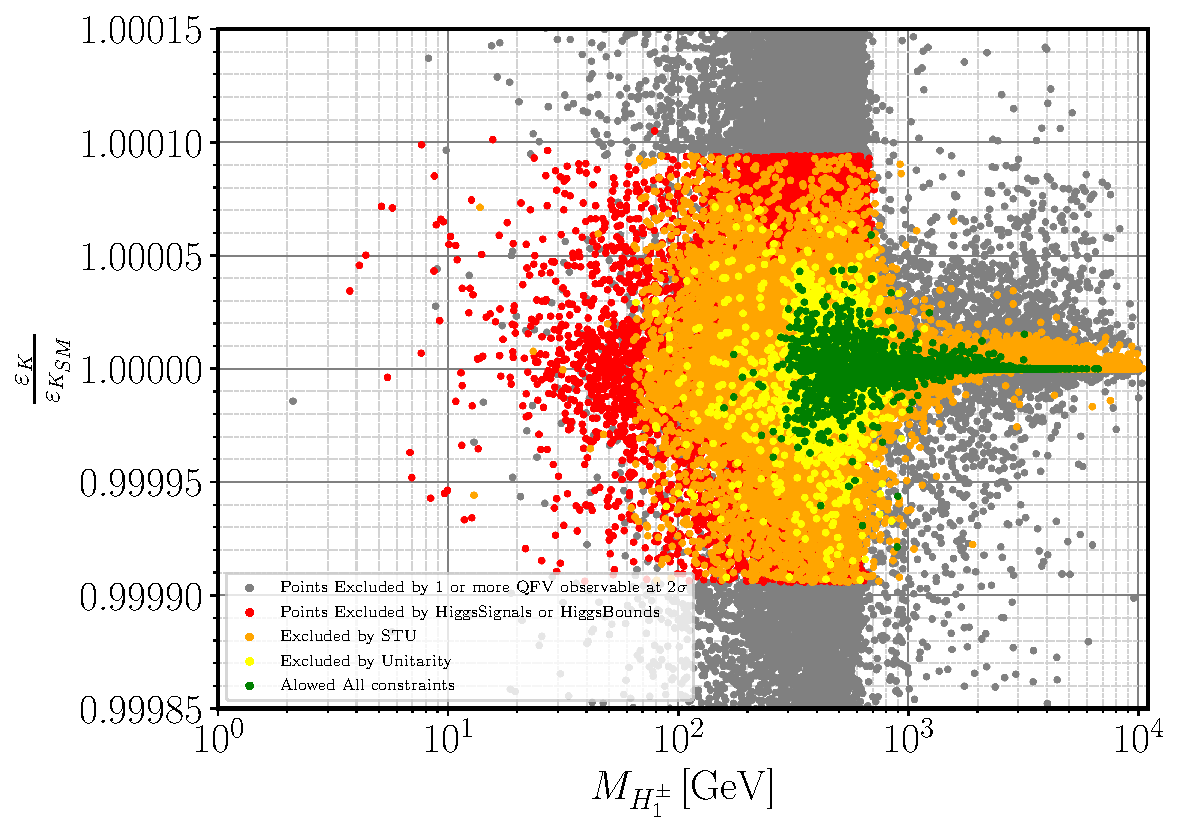
\includegraphics[width=.75\textwidth]{/3HDM/Eps_K_Hc1_Thighter_Centered.pdf}
	\caption{}
	\label{fig:STU_3}
\end{figure}	

\subsubsection{Fine-Tuning}


\subsection{Conclusions}
 
New scalars with masses below
the TeV scale can still successfully negotiate the constraints arising from flavour data.

\section{Old}

We have studied the main features and the phenomenological  consistency of a family non-universal Three Higgs Doublet Model or 3HDM with a softly broken $\mathrm{U(1)\times Z_2} $ symmetry group. This broken symmetry will justify the flavour hierarchies in the SM and trough a Branco-Grimus-Lavoura mechanism supress the otherwise expected Flavour Changing Neutral Currents. 

Let us now consider an extended version of the SM, with an enlarged Higgs sector that contains three generations of scalar-doublets. These Higgs will be named $\phi^i$ with $i={1,2,3}$.  In this sector we must enforce the alignment limit to the scalar sector ensuring the physical scalar spectrum accommodates a SM-like Higgs boson with mass of $125.09$ GeV.